%%%%%%%%%%%%%%%%%%%%%%%%%%%%%%%%%%%%%%%%%%%%%%
%% Compile: XeLaTeX BibTeX XeLaTeX XeLaTeX
%% Handout: Antonio Machicao y Priemer
%% Course: GK Linguistik
%%%%%%%%%%%%%%%%%%%%%%%%%%%%%%%%%%%%%%%%%%%%%%

%\documentclass[a4paper,10pt, bibtotoc]{beamer}
\documentclass[10pt,handout]{beamer}

%%%%%%%%%%%%%%%%%%%%%%%%
%%     PACKAGES & COMMANDS
%%%%%%%%%%%%%%%%%%%%%%%%

%%%%%%%%%%%%%%%%%%%%%%%%
%%     PACKAGES       %%
%%%%%%%%%%%%%%%%%%%%%%%%



%\usepackage[utf8]{inputenc}
%\usepackage[vietnamese, english,ngerman]{babel}   % seems incompatible with german.sty
%\usepackage[T3,T1]{fontenc} breaks xelatex

\usepackage{lmodern}
\usepackage{calligra}

\usepackage{amsmath}
\usepackage{amsfonts}
\usepackage{amssymb}
%% MnSymbol: Mathematische Klammern und Symbole (Inkompatibel mit ams-Packages!)
%% Bedeutungs- und Graphemklammern: $\lsem$ Tisch $\rsem$ $\langle TEXT \rangle$ $\llangle$ TEXT $\rrangle$ 
\usepackage{MnSymbol}
%% ulem: Strike out
\usepackage[normalem]{ulem}  

%% Special Spaces (s. Commands)
\usepackage{xspace}				
\usepackage{setspace}
%	\onehalfspacing

%% mdwlist: Special lists
\usepackage{mdwlist}	


%%%%%%%%%%%%%%%%%%%%%%%%%%%%%%%%
%% TIPA & Phonetics

\usepackage[
%noenc,
safe]{tipa}

%% TIPA Problems/Solutions:
%% Problems with U, serif fonts and ligatures

%%Test 1
%\DeclareFontSubstitution{T3}{cmss}{m}{n}

%%Test 2
%\DeclareFontSubstitution{T3}{ptm}{m}{n}

%%Test 3
%\usepackage{tipx}


%\usepackage{vowel}


%%%%%%%%%%%%%%%%%%%%%%%%%%%%%%%%
%% Examples

\usepackage{jambox}



%\usepackage{forest-v105}
%\usepackage{langsci-forest-v105-setup}


%%%%%%%%%%%%%%%%%%%%%%%%%%%%%%%%
%% Fonts for Chinese, Vietnamese, etc. (s. Graphematik)

\usepackage{xeCJK}
\setCJKmainfont{SimSun}


%\usepackage{natbib}
%\setcitestyle{notesep={:~}}


% for toggles, is loaded in hu-beamer-includes-pdflatex
%\usepackage{etex}


%%%%%%%%%%%%%%%%%%%%%%%%%%%%%%%%
%% Fonts for Fraktur

\usepackage{yfonts}

\usepackage{url}

% für UDOP
\usepackage{adjustbox}


%% huberlin: Style sheet
%\usepackage{huberlin}
\usepackage{hu-beamer-includes-pdflatex}
\huberlinlogon{0.86cm}

% %% % use this definition, if you want to see the outlines in the handout
\renewcommand{\outline}[1]{%
%\beamertemplateemptyfootbar%
\huberlinjustbarfootline
\frame{\frametitle{\outlineheading}#1}%
%\beamertemplatecopyrightfootframenumber%
\huberlinnormalfootline 
\huberlinpagedec
}



%% Last Packages
%\usepackage{hyperref}	%URLs
%\usepackage{gb4e}		%Linguistic examples

% sorry this was incompatible with gb4e and had to go.
%\usepackage{linguex-cgloss}	%Linguistic examples (patched version that works with jambox

\usepackage{multirow}  %Mehrere Zeilen in einer Tabelle
\usepackage{adjustbox} %adjusting tables
%\usepackage{array}
\usepackage{marginnote}	%Notizen




%%%%%%%%%%%%%%%%%%%%%%%%%%%%%%%%%%%%%%%%%%%%%%%%%%%%
%%%            MyP-Commands                     
%%%%%%%%%%%%%%%%%%%%%%%%%%%%%%%%%%%%%%%%%%%%%%%%%%%%


%%%%%%%%%%%%%%%%%%%%%%%%%%%%%%%%
% Delete Caption from Figures and Tables
\setbeamertemplate{caption}{\centering\insertcaption\par }


%%%%%%%%%%%%%%%%%%%%%%%%%%%%%%%%
% German quotation marks:
\newcommand{\gqq}[1]{\glqq{}#1\grqq{}}		%double
\newcommand{\gq}[1]{\glq{}#1\grq{}}			%simple


%%%%%%%%%%%%%%%%%%%%%%%%%%%%%%%%
% Abbreviations in German
% package needed: xspace
% Short space in German abbreviations: \,	
\newcommand{\idR}{\mbox{i.\,d.\,R.}\xspace}
\newcommand{\su}{\mbox{s.\,u.}\xspace}
%\newcommand{\ua}{\mbox{u.\,a.}\xspace}       % in abbrev
\newcommand{\vgl}{\mbox{vgl.}\xspace}       % in abbrev
%\newcommand{\zB}{\mbox{z.\,B.}\xspace}       % in abbrev
%\newcommand{\s}{s.~}
%not possibel: \dh --> d.\,h.

%rot unterstrichen
%\newcommand{\rotul}[1]{\textcolor{red}{\underline{#1}}}

%%%%%%%%%%%%%%%%%%%%%%%%%%%%%%%%
%Abbreviations in English
\newcommand{\ao}{a.o.\ }	% among others
%\newcommand{\cf}[1]{(cf.~#1)}	% confer = compare
\renewcommand{\ia}{i.a.}	% inter alia = among others
%\newcommand{\ie}{i.e.~}	% id est = that is
\newcommand{\fe}{e.g.~}	% exempli gratia = for example
%not possible: \eg --> e.g.~
\newcommand{\vs}{vs.\ }	% versus
\newcommand{\wrt}{w.r.t.\ }	% with respect to


%%%%%%%%%%%%%%%%%%%%%%%%%%%%%%%%
% Dash:
\newcommand{\gs}[1]{--\,#1\,--}


%%%%%%%%%%%%%%%%%%%%%%%%%%%%%%%%
% Rightarrow with and without space
\def\ra{\ensuremath\rightarrow}			%without space
\def\ras{\ensuremath\rightarrow\ }		%with space


%%%%%%%%%%%%%%%%%%%%%%%%%%%%%%%%
%% X-bar notation

%% Notation with primes (not emphasized): \xbar{X}
\newcommand{\MyPxbar}[1]{#1$^{\prime}$}
\newcommand{\xxbar}[1]{#1$^{\prime\prime}$}
\newcommand{\xxxbar}[1]{#1$^{\prime\prime\prime}$}

%% Notation with primes (emphasized): \exbar{X}
\newcommand{\exbar}[1]{\emph{#1}$^{\prime}$}
\newcommand{\exxbar}[1]{\emph{#1}$^{\prime\prime}$}
\newcommand{\exxxbar}[1]{\emph{#1}$^{\prime\prime\prime}$}

% Notation with zero and max (not emphasized): \xbar{X}
\newcommand{\zerobar}[1]{#1$^{0}$}
\newcommand{\maxbar}[1]{#1$^{\textsc{max}}$}

% Notation with zero and max (emphasized): \xbar{X}
\newcommand{\ezerobar}[1]{\emph{#1}$^{0}$}
\newcommand{\emaxbar}[1]{\emph{#1}$^{\textsc{max}}$}

%% Notation with bars (already implemented in gb4e):
% \obar{X}, \ibar{X}, \iibar{X}, \mbar{X} %Problems with \mbar!
%
%% Without gb4e:
\newcommand{\overbar}[1]{\mkern 1.5mu\overline{\mkern-1.5mu#1\mkern-1.5mu}\mkern 1.5mu}
%
%% OR:
\newcommand{\MyPibar}[1]{$\overline{\textrm{#1}}$}
\newcommand{\MyPiibar}[1]{$\overline{\overline{\textrm{#1}}}$}
%% (emphasized):
\newcommand{\eibar}[1]{$\overline{#1}$}
\newcommand{\eiibar}[1]{\overline{$\overline{#1}}$}

%%%%%%%%%%%%%%%%%%%%%%%%%%%%%%%%
%% Subscript & Superscript: no italics
\newcommand{\MyPdown}[1]{\textsubscript{#1}}
\newcommand{\MyPup}[1]{\textsuperscript{#1}}

%%%%%%%%%%%%%%%%%%%%%%%%%%%%%%%%
%% Small caps subscripts & superscripts
\newcommand{\scdown}[1]{\textsubscript{\textsc{#1}}}
\newcommand{\scup}[1]{\textsuperscript{\textsc{#1}}}

%%%%%%%%%%%%%%%%%%%%%%%%%%%%%%%%
% Objekt language marking:
%\newcommand{\obj}[1]{\glqq{}#1\grqq{}}	%German double quotes
%\newcommand{\obj}[1]{``#1''}			%English double quotes
%\newcommand{\MyPobj}[1]{\emph{#1}}		%Emphasising
\newcommand{\MyPobj}[1]{\textit{#1}}		%Emphasising

%%%%%%%%%%%%%%%%%%%%%%%%%%%%%%%%
% Size:
\newcommand{\size}[1]{#1}	% f.e. resize citations


%%%%%%%%%%%%%%%%%%%%%%%%%%%%%%%%
%% Semantic types (<e,t>), features, variables and graphemes in angled brackets 

%%% types and variables, in math mode: angled brackets + italics + no space
%\newcommand{\type}[1]{$<#1>$}

%%% OR more correctly: 
%%% types and variables, in math mode: chevrons! + italics + no space
\newcommand{\MyPtype}[1]{$\langle #1 \rangle$}

%%% features and graphemes, in math mode: chevrons! + italics + no space
\newcommand{\abe}[1]{$\langle #1 \rangle$}


%%% features and graphemes, in math mode: chevrons! + no italics + space
\newcommand{\ab}[1]{$\langle$#1$\rangle$}  %%same as \abu  
\newcommand{\abu}[1]{$\langle$#1$\rangle$} %%Umlaute


%% Presuppositions
\newcommand{\prspp}{$\gg$} 

%% Implicature
\newcommand{\implc}{$+ \mkern-5mu >$} 

%% Enttailment
\newcommand{\ent}{$\vDash$}

%% Other semantic symbols: 
%% entailment: $\Rightarrow$ $\vDash$
%% equivalence: $\Leftrightarrow$ $\equiv$
%% biconditional: $\leftrightarrow$ 
%% lexical rule: $\mapsto$
%% greater/less/equal: $>$ $\geq$ $<$ $\leq$
%% definition: $:=$ $=$\textsubscript{def}


%%%%%%%%%%%%%%%%%%%%%%%%%%%%%%%%
% Marking text with colour:
% package needed: xcolor
% Command \alert{} in Beamer >> FU-grün (leider!! @Stefan)

%%%neue Farbbefehle in Anlehnung an rotul
%%%(s. hu-beamer-includes-pdflatex.sty in texmf)

%% Farbdefinitionen:

\definecolor{HUred}{RGB}{138,15,20}
\definecolor{HUblue}{RGB}{0,55,108}
\definecolor{HUgreen}{RGB}{0,87,44}

%\newcommand{\alertred}[1]{\textcolor{red}{#1}}  % basic red
\newcommand<>{\alertred}[1]{{\color#2[RGB]{138,15,20}#1}}  %HU rot + overlay

%\newcommand{\alertblue}[1]{\textcolor{blue}{#1}} 		% basic blue
\newcommand<>{\alertblue}[1]{{\color#2[RGB]{0,55,108}#1}} %HU blue + overlay

%\newcommand{\alertgreen}[1]{\textcolor{green}{#1}}	% basic green
\newcommand<>{\alertgreen}[1]{{\color#2[RGB]{0,87,44}#1}} %HU green + overlay


%%% Verwendung der oben definierten Farben mit Unterschied in Handout und Beamer:

\mode<handout>{%
	\newcommand<>{\hured}[1]{\only#2{\underline{#1}}}
	\newcommand<>{\hublue}[1]{\only#2{\textbf{#1}}}
	\newcommand<>{\hugreen}[1]{\only#2{\textsc{#1}}}
}
%
\mode<beamer>{%
	\newcommand<>{\hured}[1]{\alertred#2{#1}}
	\newcommand<>{\hublue}[1]{\alertblue#2{#1}}
	\newcommand<>{\hugreen}[1]{\alertgreen#2{#1}}
}


%%%%%%%%%%%%%%%%%%%%%%%%%%%%%%%%
%% Outputbox
\newcommand{\outputbox}[1]{\noindent\fbox{\parbox[t][][t]{0.98\linewidth}{#1}}\vspace{0.5em}}


%%%%%%%%%%%%%%%%%%%%%%%%%%%%%%%%
%% (Syntactic) Trees
% package needed: forest
%
%% Setting for simple trees
\forestset{
	MyP edges/.style={for tree={parent anchor=south, child anchor=north}}
}

%% this is taken from langsci-setup file
%% Setting for complex trees
%% \forestset{
%% 	sm edges/.style={for tree={parent anchor=south, child anchor=north,align=center}}, 
%% background tree/.style={for tree={text opacity=0.2,draw opacity=0.2,edge={draw opacity=0.2}}}
%% }

\newcommand\HideWd[1]{%
	\makebox[0pt]{#1}%
}

%%%%%%%%%%%%%%%%%%%%%%%%%%%%%%%
%%solutions in green + w/ jambox
\newcommand{\loesung}[2]{\jambox{\visible<#1->{\alertgreen{#2}}}}

%%%%%%%%%%%%%%%%%%%%%%%%%%%%%%%%
%% TIPA Lösungen           

%%Tipa serif font fixed (requires package 'Linux Libertine B')

%% Solution 1 (RF)
%% Tipa font:
%\renewcommand\textipa[1]{{\fontfamily{cmr}\tipaencoding #1}}

%% Solution 2 (RF): older code for texlive 2017?
%\newfontfamily{\tipacm}[Scale=MatchUppercase]{Linux Libertine B}
%\renewcommand\useTIPAfont{\tipacm}

%\NewEnviron{IPA}{\expandafter\textipa\expandafter{\BODY}} %% not needed anymore

%% Solution 3 (RF): this solution is working but with problems with ligatures
%%% works for texlive 2018
\newfontfamily{\ipafont}[Scale=MatchUppercase]{Linux Libertine B}
\def\useTIPAfont{\ipafont}

%% Solution 4 (Kopecky & MyP): Test package: tipx (s. localpackages) and comment "Solution 3" 


%%%%%%%%%%%%%%%%%%%%%%%%%%%%%%%%
%% Toggles                  


\newtoggle{uebung}
\newtoggle{loesung}\togglefalse{loesung}

\newtoggle{hausaufgabe}

%\newtoggle{ha-loesung}\togglefalse{ha-loesung}
\newtoggle{phonologie-loesung}
\newtoggle{graphematik-loesung}


%% Neue Toggle-Struktur
\newtoggle{toc}
\newtoggle{sectoc}
\newtoggle{gliederung}

\newtoggle{ue-loesung}
\newtoggle{ha-loesung}
%%

% The toc is not needed on Handouts. Save trees.
\mode<handout>{
\togglefalse{toc}
}

\newtoggle{hpsgvorlesung}\togglefalse{hpsgvorlesung}
\newtoggle{syntaxvorlesungen}\togglefalse{syntaxvorlesungen}

%\includecomment{psgbegriffe}
%\excludecomment{konstituentenprobleme}
%\includecomment{konstituentenprobleme-hinweis}

\newtoggle{konstituentenprobleme}\togglefalse{konstituentenprobleme}
\newtoggle{konstituentenprobleme-hinweis}\toggletrue{konstituentenprobleme-hinweis}

%\includecomment{einfsprachwiss-include}
%\excludecomment{einfsprachwiss-exclude}
\newtoggle{einfsprachwiss-include}\toggletrue{einfsprachwiss-include}
\newtoggle{einfsprachwiss-exclude}\togglefalse{einfsprachwiss-exclude}

\newtoggle{psgbegriffe}\toggletrue{psgbegriffe}

\newtoggle{gb-intro}\togglefalse{gb-intro}


%%%%%%%%%%%%%%%%%%%%%%%%%%%%%%%%
%% Useful commands                    

%%%%%%%%%%%%%%%%%%%%%
%% FOR ITEMS:
%\begin{itemize}
%  \item<2-> from point 2
%  \item<3-> from point 3 
%  \item<4-> from point 4 
%\end{itemize}
%
% or: \onslide<2->
% or \only<2->{Text}
% or: \pause

%%%%%%%%%%%%%%%%%%%%%
%% VERTICAL SPACE:
% \vspace{.5cm}
% \vfill

%%%%%%%%%%%%%%%%%%%%%
% RED MARKING OF TEXT:
%\alert{bis spätestens Mittwoch, 18 Uhr}
%\newcommand{\alertred}[1]{\textcolor{red}{#1}}

%%%%%%%%%%%%%%%%%%%%%
%% RESCALE BIG TABLES:
%\scalebox{0.8}{
%For Big Tables
%}

%%%%%%%%%%%%%%%%%%%%%
%% BLOCKS:
%\begin{alertblock}{Title}
%Text
%\end{alertblock}
%
%\begin{block}{Title}
%Text
%\end{block}
%
%\begin{exampleblock}{Title}
%Text
%\end{exampleblock}

%%%%%%%%%%%%%%%%%%%%%
%% JAMBOX FOR EXAMPLES:
%\ea 
%\settowidth\jamwidth{Test} 
%Die Studierenden, die weitgehend von Stipendien leben, erhalten einen Mietzuschuss. 
%\jambox{Test}
%\z 

%%%%%%%%%%%%%%%%%%%%%
%% TOGGLES:


%%%%%%%%%%%%%%%%%%%%%%%%%%%%%%%%%%
%%%%%%%%%%%%%%%%%%%%%%%%%%%%%%%%%%
%\subsection{Übung}
%
%%%%%%%%%%%%%%%%%%%%%%%%%%%%%%%%%%
%%%%%%%%%%%%%%%%%%%%%%%%%%%%%%%%%%
%\iftoggle{uebung}{
%%%%%%%%%%%%%%%%%%%%%%%%%%%%%%%%%%
%\begin{frame}
%\frametitle{Übung}
%
%\end{frame}
%
%} 
%%% END true = Q
%%% BEGIN false = Q + A
%{
%%%%%%%%%%%%%%%%%%%%%%%%%%%%%%%%%%
%\begin{frame}
%\frametitle{Übung}
%
%\end{frame}
%%%%%%%%%%%%%%%%%%%%%%%%%%%%%%%%%%
%
%\begin{frame}
%\frametitle{Lösung}
%
%\end{frame}
%
%}%% END LOESUNG	
%%%%%%%%%%%%%%%%%%%%%%%%%%%%%%%%%%


%%%%%%%%%%%%%%%%%%%%%%%%%%%%%%%%%%
%%%%%%%%%%%%%%%%%%%%%%%%%%%%%%%%%%
%\subsection{Hausaufgabe}
%
%%%%%%%%%%%%%%%%%%%%%%%%%%%%%%%%%%
%%%%%%%%%%%%%%%%%%%%%%%%%%%%%%%%%%
%\iftoggle{hausaufgabe}{
%%%%%%%%%%%%%%%%%%%%%%%%%%%%%%%%%%
%
%\begin{frame}
%\frametitle{Hausaufgabe}
%
%\end{frame}
%
%} 
%%% END true = Q
%%% BEGIN false = Q + A
%{
%%%%%%%%%%%%%%%%%%%%%%%%%%%%%%%%%%
%
%\begin{frame}
%\frametitle{Hausaufgabe}
%
%\end{frame}
%
%
%%%%%%%%%%%%%%%%%%%%%%%%%%%%%%%%%%
%%%%%%%%%%%%%%%%%%%%%%%%%%%%%%%%%%
%\subsection*{Lösung der Hausaufgabe}
%
%%%%%%%%%%%%%%%%%%%%%%%%%%%%%%%%%%
%
%\begin{frame}
%\frametitle{Lösung}
%
%\end{frame}
%
%}%% END LOESUNG	
%%%%%%%%%%%%%%%%%%%%%%%%%%%%%%%%%%



%%%%%%%%%%%%%%%%%%%%%%%%%%%%%%%%%%%%%%%%%%%%%%%%%%%%
%%%             Preamble's End                   
%%%%%%%%%%%%%%%%%%%%%%%%%%%%%%%%%%%%%%%%%%%%%%%%%%%% 

\begin{document}
	
	
%%%% ue-loesung
%%%% true: Übung & Lösungen (slides) / false: nur Übung (handout)
	\togglefalse{ue-loesung}

%%%% ha-loesung
%%%% true: Hausaufgabe & Lösungen (slides) / false: nur Hausaufgabe (handout)
	\togglefalse{ha-loesung}

%%%% toc
%%%% true: TOC am Anfang von Slides / false: keine TOC am Anfang von Slides
\toggletrue{toc}

%%%% sectoc
%%%% true: TOC für Sections / false: keine TOC für Sections (StM handout)
\toggletrue{sectoc}

%%%% gliederung
%%%% true: Gliederung für Sections / false: keine Gliederung für Sections
%	\toggletrue{gliederung}


%%%%%%%%%%%%%%%%%%%%%%%%%%%%%%%%%%%%%%%%%%%%%%%%
%% Compile the master file!
%% 		Slides: Antonio Machicao y Priemer
%% 		Course: GK Linguistik
%%%%%%%%%%%%%%%%%%%%%%%%%%%%%%%%%%%%%%%%%%%%%%%%


%%%%%%%%%%%%%%%%%%%%%%%%%%%%%%%%%%%%%%%%%%%%%%%%%%%%
%%%             Metadata                         
%%%%%%%%%%%%%%%%%%%%%%%%%%%%%%%%%%%%%%%%%%%%%%%%%%%%      

\title{Grundkurs Linguistik}

\subtitle{Phonologie I}

\author[A. Machicao y Priemer]{
	{\small Antonio Machicao y Priemer}
	\\
	{\footnotesize \url{http://www.linguistik.hu-berlin.de/staff/amyp}}
	%	\\
	%	\href{mailto:mapriema@hu-berlin.de}{mapriema@hu-berlin.de}}
}

\institute{Institut für deutsche Sprache und Linguistik}


% bitte lassen, sonst kann man nicht sehen, von wann die PDF-Datei ist.
%\date{ }

%\publishers{\textbf{6. linguistischer Methodenworkshop \\ Humboldt-Universität zu Berlin}}

%\hyphenation{nobreak}


%%%%%%%%%%%%%%%%%%%%%%%%%%%%%%%%%%%%%%%%%%%%%%%%%%%%
%%%             Preamble's End                  
%%%%%%%%%%%%%%%%%%%%%%%%%%%%%%%%%%%%%%%%%%%%%%%%%%%%      


%%%%%%%%%%%%%%%%%%%%%%%%%      
\huberlintitlepage[22pt]

\iftoggle{toc}{
\frame{
%\begin{multicols}{2}
	\frametitle{Inhaltsverzeichnis}
	\tableofcontents
	%[pausesections]
%\end{multicols}
}
}

%%%%%%%%%%%%%%%%%%%%%%%%%%%%%%%%%%
%%%%%%%%%%%%%%%%%%%%%%%%%%%%%%%%%%
%%%%%LITERATURE:

%% Allgemein
\nocite{Glueck&Roedel16a}
\nocite{Schierholz&Co18}
\nocite{Luedeling2009a}
\nocite{Meibauer&Co07a} 
\nocite{Repp&Co15a} 

%%% Sprache & Sprachwissenschaft
%\nocite{Fries16c} %Adäquatheit
%\nocite{Fries16a} %Grammatikalität
%\nocite{Fries&MyP16c} %GG
%\nocite{Fries&MyP16b} %Akzeptabilität
\nocite{Fries&MyP16d} %Kompetenz vs. Performanz

%% Phonetik & Phonologie
\nocite{Altmann&Co07a}
\nocite{DudenAussprache00a}
\nocite{Hall00a} 
\nocite{Kohler99a}
\nocite{Krech&Co09a}
\nocite{Pompino95a}
\nocite{Ramers08a}
\nocite{Ramers&Vater92a}
\nocite{Rues&Co07a}
\nocite{WieseR11a}


%%%%%%%%%%%%%%%%%%%%%%%%%%%%%%%%%%%
%%%%%%%%%%%%%%%%%%%%%%%%%%%%%%%%%%%
\section{Phonologie}

%%%%%%%%%%%%%%%%%%%%%%%%%%%%%%%%%%%
%%%%%%%%%%%%%%%%%%%%%%%%%%%%%%%%%%%
\begin{frame}
\frametitle{Begleitlektüre}

	\begin{itemize}
		\item \textbf{obligatorisch:}
		\begin{itemize}
			\item[] AM S.~13--18
		\end{itemize}
		\item \textbf{optional:}
		\begin{itemize}
			\item[] \citet{Hall00a}: Kapitel 2 (S.~37--47; 62--72)  
		\end{itemize}
	\end{itemize}

\end{frame}


%%%%%%%%%%%%%%%%%%%%%%%%%%%%%%%%%%%
\subsection{Einführung}

%%MyP: Contents
\iftoggle{sectoc}{
	\frame{
		%		\begin{multicols}{2}
		\frametitle{~}
		\tableofcontents[currentsubsection,subsubsectionstyle=hide]
		%		\end{multicols}
	}
}

%% StM: Contents
\iftoggle{gliederung}{
	
	\outline{
		\begin{itemize}
			
			\item \blaubf{Einführung}
			\item Phonem, Phon, Allophon
			\item Phonetisch-phonologische Ebenen
			\item Phonetisch-phonologische Prozesse
			\item Hausaufgabe
			
		\end{itemize}
	}
}
%%%%%%%%%%%%%%%%%%%%%%%%%%%%%%%%%%%
\begin{frame}{Einführung}

\begin{itemize}
	\item  Phonologie, auch \textbf{Sprachgebilde}lautlehre
	\item  Phonetik, auch \textbf{Sprechakt}lehre
	\item Trennung von Phonetik und Phonologie: Ende der 1920er Jahre
	\item Strukturalistische Lehre der Prager Schule \citep[vgl.][]{Trubetzkoy89a-doppelt}

	\bigskip
	\pause
	\item Unterscheidung auf allen Ebenen zwischen:
	
	\begin{itemize}
		\item Sprachgebilde: \textbf{zugrunde liegendes System}: \textit{langue} \\
		(ab \citet{Chomsky65a}: \textit{Kompetenz})

		\medskip 

		\item[] und

		\medskip 

		\item Sprechakt: \textbf{tatsächliche Realisierung} in einer Kommunikationssituation: \textit{parole}\\
		 (ab \citet{Chomsky65a}: \textit{Performanz})
	\end{itemize}
	
\end{itemize}

\end{frame}



%%%%%%%%%%%%%%%%%%%%%%%%%%%%%%%%%%%
\begin{frame}
\frametitle{Phonetik \vs Phonologie}

\begin{itemize}
	\item \textbf{Phonetik:} Untersuchung der materiellen Seite des Sprechens (Phone)
	\item[]
	\item \textbf{Phonologie:} Systematik der Laute \ras Materielle (messbare) Daten der Phonetik werden in abstrakterer Art und Weise \textbf{systematisiert}
	
\end{itemize}

\end{frame}



%%%%%%%%%%%%%%%%%%%%%%%%%%%%%%%%%%%
\begin{frame}
\frametitle{Untersuchungsgegenstände der Phonologie -- I}
	
	\begin{itemize}
		\item \textbf{Phoneminventar}: bedeutungsunterscheidende Laute einer Sprache 

		\ea Im Dt. bedeutungsunterscheidend \textipa{[v]} und \textipa{[f]}: \\
		\textipa{[v\t{aI}n]} vs.\ \textipa{[f\t{aI}n]} (Wein, fein)
	\z
	
		\item Deutsch: 16 Vokale \& 20 Konsonanten
		\item Rotokas (Papua): 5 Vokale \& 6 Konsonanten
		\item Mittelwert:  8 Vokale \& 23 Konsonanten
	
		\item \textbf{Allophonie}: Vorkommen vs. Nicht-Vorkommen (bzw. Variation) von Lauten in bestimmten Kontexten

		\ea Wann kommt der \gqq{Ich-Laut} und wann der \gqq{Ach-Laut} vor?
		\z

\end{itemize}

\end{frame}


%%%%%%%%%%%%%%%%%%%%%%%%%%%%%%%%%%%
\begin{frame}
\frametitle{Untersuchungsgegenstände der Phonologie -- II}

\begin{itemize}

		\item \textbf{Phonologische Distribution}:\par
		An welchen Stellen kann ein Laut oder eine Lautfolge auftreten?

	\ea \textipa{[St\textscr]} am Wortanfang aber nicht am Wortende:\\
	\textipa{[St{\textscr}\t{aU}x]} \vs *\textipa{[\ldots aSt\textscr]}
	\z
	
	\item Phoneminventar, phonologische Distribution und Allophonie werden in der \textbf{strukturalistischen Phonologie} untersucht.

\end{itemize}

\begin{block}{Strukturalistische Phonologie}
	Beschreibung von sprachlichen Daten 
\end{block}

\end{frame}


%%%%%%%%%%%%%%%%%%%%%%%%%%%%%%%%%%%
\begin{frame}
\frametitle{Untersuchungsgegenstände der Phonologie -- III}
	
\begin{itemize}		
	\item \textbf{Phonologische Prozesse}: Welche Lautfolgen, die an der Oberfläche unterschiedlich klingen, werden durch die Sprachnutzer trotzdem als Varianten eines zugrunde liegenden Musters erkannt?

\ea \textipa{[ga{\textscr}t@n]} kann als \textipa{[ga:d\textsyllabic{n}]} ausgesprochen werden aber nicht als 
\textipa{[ga:b\s{m}]}
\z

\end{itemize}


\begin{block}{Generative Phonologie}
	Untersuchung der zugrunde liegenden Form und der (generativen) Regeln, um Schlüsse über die \textbf{allgemeine Sprachfähigkeit} zu ziehen
\end{block}

      
\begin{itemize}

\item Aufgaben des \textbf{phonologischen Moduls}:
	
	\begin{itemize}
		\item Bildung (und Verständnis) wohlgeformter Lautketten
		\item Inventar von Minimaleinheiten (distinktive Merkmale -- hier Phoneme!)
		\item Regelinventar
	\end{itemize}
	 
\end{itemize}

\end{frame}


%%%%%%%%%%%%%%%%%%%%%%%%%%%%%%%%%%%
\begin{frame}
\frametitle{Weitere Untersuchungsgebiete der Phonologie}

	\begin{itemize}
		\item Eigenschaften von (lautlichen) Einheiten, die größer sind als ein Laut (\zB~\textbf{Silbenphonologie})
		\item Wortakzent (\textbf{metrische Phonologie})
		\item Satzakzent, Phrasierung, Pausen, Sprechmelodie (\textbf{prosodische Phonologie}, Intonation)
		\item Betrachtung der Laute (\textbf{lineare Phonologie})
		\item Analyse einer Silbe (\textbf{nicht-lineare/hierarchische Phonologie})

	\end{itemize}


\begin{block}{Lineare Phonologie}
Untersuchung der Segmente (Laute) und ihrer unmittelbaren Kontexte
\end{block}

\begin{block}{Hierarchische (nicht-lineare) Phonologie}
Untersuchung der suprasegmentalen Ebene (\zB Silbe)
\end{block}
\end{frame}


%%%%%%%%%%%%%%%%%%%%%%%%%%%%%%%%%%%
%%%%%%%%%%%%%%%%%%%%%%%%%%%%%%%%%%%
\subsection{Phonem, Phon, Allophon}

%%MyP: Contents
\iftoggle{sectoc}{
	\frame{
		%		\begin{multicols}{2}
		\frametitle{~}
		\tableofcontents[currentsubsection,subsubsectionstyle=hide]
		%		\end{multicols}
	}
}

%% StM: Contents
\iftoggle{gliederung}{
	
	\outline{
		\begin{itemize}
			
			\item Einführung
			\item \blaubf{Phonem, Phon, Allophon}
			\item Phonetisch-phonologische Ebenen
			\item Phonetisch-phonologische Prozesse
			\item Hausaufgabe
			
		\end{itemize}
	}
}
%%%%%%%%%%%%%%%%%%%%%%%%%%%%%%%%%%%

\begin{frame}{Phonem, Phon, Allophon}

\begin{itemize}
	\item \textbf{Phon} (Notation \textipa{[ ]}):
	
	\begin{itemize}
		%\item[]
		\item Minimaleinheit der Phonetik
		\item physikalisch messbare lautliche Einheit einer Sprache
	\end{itemize}
	
	\item \textbf{Phonem} (Notation \textipa{/ /}):
	
	\begin{itemize}
		%\item[]
		\item Minimaleinheit der Phonologie
		\item abstraktes Konstrukt, steht für eine \textbf{Menge} von möglichen Phonen (Allophonen)
		\item Resultat von \textbf{Systematisierung}
		\item ermittelbar durch \textbf{Minimalpaarbildung} (strukturalistisches Kriterium)	
	\end{itemize}
	
\end{itemize}

\end{frame}


%%%%%%%%%%%%%%%%%%%%%%%%%%%%%%%%%%%
\begin{frame}
\frametitle{Phonem}

	\begin{itemize}
	
		\item ermittelbar durch \textbf{Minimalpaarbildung} (strukturalistisches Kriterium)
		
		\begin{block}{Minimalpaar}
			Wortpaar, das sich nur in einem Laut (eher Phonem) an der gleichen Stelle unterscheidet
		\end{block}
	
	\eal
		\ex \label{schaf} \textipa{[Sa:l]}  \ab{Schal} vs. \textipa{[Sa:f]} \ab{Schaf} \ras \textipa{/l/} \vs \textipa{/f/}
		\ex\label{schall} \textipa{[Sa:l]} \ab{Schal} vs. \textipa{[Sal]} \ab{Schall} \ras \textipa{/a:/} \vs \textipa{/a/}
		\ex \label{saal} \textipa{[Sa:l]} \ab{Schal} vs. \textipa{[za:l]} \ab{Saal} \ras \textipa{/S/} \vs \textipa{/z/}
	\zl
	
		\item \textbf{Phonologische Opposition}: Austausch der Laute wirkt sich bedeutungsunterscheidend (oder kategorieunterscheidend) aus.
	
	\eal
		\ex \textipa{/l/} vs. \textipa{/f/} in (\ref{schaf})
		\ex \textipa{/a:/} vs. \textipa{/a/} in (\ref{schall})
		\ex \textipa{/S/} vs. \textipa{/z/} in (\ref{saal})
	\zl			
	
	\end{itemize}

\end{frame}


%%%%%%%%%%%%%%%%%%%%%%%%%%%%%%%%%%%
\begin{frame}
	\frametitle{Übung}
	
Sind folgende Laute im Deutschen bedeutungsunterscheidend?\\
Finden Sie Minimalpaare:

\begin{enumerate}
	\item \textipa{[d]} \vs \textipa{[t]}
	
% Dante/Tante
\medskip

	\item \textipa{[a]} \vs \textipa{[a:]}
	
% All Aal
\medskip

	\item \textipa{[z]} \vs \textipa{[s]}
% sein Schein
\end{enumerate}


\end{frame}


%%%%%%%%%%%%%%%%%%%%%%%%%%%%%%%%%%%
\begin{frame}
\frametitle{Phonem (strukturalistisch)}

\begin{itemize}
	\item kleinste bedeutungsunterscheidende Einheit eines Sprachsystems
	\item Ein Phonem \textbf{trägt keine} Bedeutung. Es \textbf{unterscheidet} Bedeutungen.
	\item[]
	\item Phoneme sind immer Phoneme \textbf{einer Sprache/eines Systems}

	\eal
		\ex Deutsch: \textipa{[papa]} \textbf{$=$} \textipa{[p\super{h}ap\super{h}a]}
		\ex Hindi: \textipa{[pal]} (\gq{sich kümmern um}) \textbf{$\neq$} \textipa{[p\super{h}al]} (\gq{Messerblatt})
	\zl

\end{itemize}

\end{frame}


%%%%%%%%%%%%%%%%%%%%%%%%%%%%%%%%%%%
\begin{frame}%[allowframebreaks]
\frametitle{Allophon}

	\begin{itemize}
		\item phonetische Realisierungsvarianten \textbf{eines} Phonems
		
		\ea \textipa{[Sp\alertred{r}a:xe]} = \textipa{[Sp\alertred{\textscr}a:xe]} = \textipa{[Sp\alertred{K}a:xe]} \\ \ras kein Bedeutungsunterschied
		\z

		\item \textbf{komplementäre} Allophonie

	\eal
	\ex[]{
          \textipa{[x]} \vs \textipa{[\c{c}]}
          }
	\ex[]{
          \textipa{[bax]} \vs \textipa{[mI\c{c}]}
          }
	\ex[*]{
          \textipa{[mIx]} \vs *\textipa{[ba\c{c}]}
          }
	\zl
	
		\item \textbf{freie} Allophonie

		\ea \textipa{[p\super{h}as]} \vs \textipa{[pas]}
		\z
		
		\item \textbf{regionale und soziale} Variation (Unterart der freien Allophonie)

		\ea \textipa{[PIS]} \vs \textipa{[PI\c{c}]}
		\z
		
	\end{itemize}

\end{frame}


%%%%%%%%%%%%%%%%%%%%%%%%%%%%%%%%%%%
%%%%%%%%%%%%%%%%%%%%%%%%%%%%%%%%%%%
\subsection{Phonetisch-phonologische Ebenen}

%%MyP: Contents
\iftoggle{sectoc}{
	\frame{
		%		\begin{multicols}{2}
		\frametitle{~}
		\tableofcontents[currentsubsection,subsubsectionstyle=hide]
		%		\end{multicols}
	}
}

%% StM: Contents
\iftoggle{gliederung}{
	
	\outline{
		\begin{itemize}
			
			\item Einführung
			\item Phonem, Phon, Allophon
			\item \blaubf{Phonetisch-phonologische Ebenen}
			\item Phonetisch-phonologische Prozesse
			\item Hausaufgabe
			
		\end{itemize}
	}
}
%%%%%%%%%%%%%%%%%%%%%%%%%%%%%%%%%%%

\begin{frame}{Phonetisch-phonologische Ebenen}

	\begin{itemize}
		\item Unterscheidung von (mindestens) zwei Ebenen
		\item[$\rightarrow$] \textipa{[\textscr a:\alertred{t}]} und \textipa{[\textscr E:\alertred{d}5]} (für \ab{Rad} und \abu{Räder})\\
		aber\\
		\textipa{[\textscr a:\alertred{t}]} und \textipa{[\textscr E:\alertred{t}@]} (für \ab{Rat} und \abu{Räte})
		\item[]
		\item[$\rightarrow$] Warum verstehen wir dasselbe, wenn wir\\
		\textipa{[ha:k@\alertred{n}]} oder \textipa{[ha:k\alertred{N}]}\\
		hören?
		\item[]
		\item \textbf{Tiefenstruktur} (Deep Structure) vs. \textbf{Oberflächenstruktur} (Surface Structure)
	\end{itemize}
	
\end{frame}



%%%%%%%%%%%%%%%%%%%%%%%%%%%%%%%%%%%
%%%%%%%%%%%%%%%%%%%%%%%%%%%%%%%%%%%
%\subsubsection{Tiefenstruktur (TS)}
%\iftoggle{toc}{
%	\frame{
%		\begin{multicols}{2}
%			\frametitle{~}
%			\tableofcontents[currentsection]
%		\end{multicols}
%	}
%}
%%%%%%%%%%%%%%%%%%%%%%%%%%%%%%%%%%%

\begin{frame}{Tiefenstruktur (TS)}
	
\begin{itemize}
	\item \textbf{zugrunde liegende abstrakte Repräsentation} $\rightarrow$ Phoneme \textipa{/ /}
	\item[]
	\item \textbf{idiosynkratische} Form $\approx$ nicht deriviert/abgeleitet
	\item Die TS-Form kann nicht durch Regeln abgeleitet werden,\\
                sie ist idiosynkratisch und muss deshalb im Lexikon gespeichert sein.
% das ist falsch, weil etwas im Lexikon abgespeichert ist, ist es nicht unbedingt idisynkratisch. Genau andersherum.
	\item[]
	\item TS besteht aus Phonemen
	
	\eal
		\ex \textipa{/\textscr a:t/}: TS-Form von \ab{Rat}
		\ex \textipa{/\textscr a:d/}: TS-Form von \ab{Rad}
		\ex \textipa{/ha:k@n/}: TS-Form von \ab{Haken}
	\zl
	
\end{itemize}
		
\end{frame}


%%%%%%%%%%%%%%%%%%%%%%%%%%%%%%%%%%%
\begin{frame}
\frametitle{Tiefenstruktur (TS) II}

\begin{itemize}
	\item \textipa{[t]} in \textipa{[\textscr a:\alertred{t}]} (von \ab{Ra\alertred{d}}) ist ableitbar.
	\item \textipa{/d/} in \textipa{/\textscr a:\alertred{d}/} ist idiosynkratisch.
	\item[]
	\item \textipa{/t/} in \textipa{/\textscr a:\alertred{t}/} (von \ab{Ra\alertred{t}}) ist idiosynkratisch.
	\item[]
	\item Wenn das Deutsche ein neues Wort wie \ab{Code} \textipa{[koUd]} entlehnen würde,\\
              würde dieses Wort früher oder später \gqq{eingedeutscht} werden.
	
	\ea \textipa{[kOUt]} oder \textipa{[ko:t]} aber \gqq{des \textipa{[kOUd@s]}} oder \gqq{des \textipa{[ko:ts]}} 
	\z
	
\end{itemize}

\end{frame}


%%%%%%%%%%%%%%%%%%%%%%%%%%%%%%%%%%%
%%%%%%%%%%%%%%%%%%%%%%%%%%%%%%%%%%%
%\subsubsection{Oberflächenstruktur (OS)}
%\iftoggle{toc}{
%	\frame{
%		\begin{multicols}{2}
%			\frametitle{~}
%			\tableofcontents[currentsection]
%		\end{multicols}
%	}
%}
%%%%%%%%%%%%%%%%%%%%%%%%%%%%%%%%%%%

\begin{frame}{Oberflächenstruktur (OS)}

\begin{itemize}
	\item Von der abstrakten phonembasierten TS wird die sog. Oberflächenstruktur mithilfe von vorhersagbaren (phonetisch-)phonologischen Regeln deriviert.
	\item[]
	\item OS entspricht der \textbf{tatsächlichen Realisierung} durch konkrete Phone \ras \textipa{[ ]}
	\item[]
	\item Demnach gibt es viele mögliche OS-Formen, darunter auch die sog.\\
		\textbf{kanonische Aussprache} ($\approx$ Standardaussprache) (s.~\ref{ex:standard})\\
		sowie die vielen möglichen \textbf{umgangssprachlichen} Formen:
%	\item[]
%	\item Häufig wird zwischen phonologischen und phonetischen Prozessen unterschieden.

\eal
\ex \label{ex:standard} \textipa{[Pe:b@n]}
\ex \textipa{[Pe:bn]}
\ex \textipa{[Pe:bm]}
\ex \textipa{[Pe:m]}
\zl
\end{itemize}

\end{frame}


%%%%%%%%%%%%%%%%%%%%%%%%%%%%%%%%%%%
\begin{frame}%[allowframebreaks]
\frametitle{Phonetische und phonologische Prozesse}

\begin{itemize}
	\item Häufig wird zwischen phonologischen und phonetischen Prozessen unterschieden.
	\item[]
	
	\item \textbf{Phonetische Prozesse} $\rightarrow$ vom Sprachtempo und Stil abhängig
	\begin{itemize}
	\item[$\rightarrow$] Plosiveinsetzung: \textipa{/amt/} $\rightarrow$ \textipa{[Pampt]}
	\end{itemize}

	\item \textbf{Phonologische Prozesse} $\rightarrow$ systematisch und obligatorisch
	\begin{itemize}
		\item[$\rightarrow$] \textit{Ich}-/\textit{Ach}-Laut-Wechsel \textipa{[bu:x]} (von \textipa{/bu:\c{c}/}) ist ableitbar
	\end{itemize}

	\item Einen klaren Schnitt zwischen phonetischen und phonologischen Prozessen gibt es nicht:
	\begin{itemize}
		\item[$\rightarrow$] Sind g-Tilgung, Spirantisierung, Schwa-Tilgung, \dots\ phonetische oder phonologische Prozesse?
	\end{itemize}

\end{itemize}

\end{frame}



%%%%%%%%%%%%%%%%%%%%%%%%%%%%%%%%%%%
%%%%%%%%%%%%%%%%%%%%%%%%%%%%%%%%%%%
%\subsubsection{TS \& OS}
%\iftoggle{toc}{
%	\frame{
%		\begin{multicols}{2}
%			\frametitle{~}
%			\tableofcontents[currentsection]
%		\end{multicols}
%	}
%}
%%%%%%%%%%%%%%%%%%%%%%%%%%%%%%%%%%%

\begin{frame}{TS \& OS}

\begin{itemize}
	\item TS \& OS sind \textbf{theoretische Abstraktionen},
              um die Regelhaftigkeiten auf der phonologischen Ebene erklären zu können.

\pause 

	\item Ein Kind erhält als \textbf{Input im Spracherwerb} OS-Formen wie: 
	
	\ea \textipa{[\textscr a:t]} und \textipa{[\textscr E:t@]}, \textipa{[\textscr a:t]} und \textipa{[\textscr E:d5]}, \textipa{[bEt]} und \textipa{[bEt@n]}, \textipa{[ba:t]} und \textipa{[bE:d5]}, \textipa{[kInt]} und \textipa{[kInd5]}
	\z 

\pause 

	\item Daraus erkennt das Kind,

	\begin{itemize}
		\item dass in einigen Wörtern \textipa{[d]} und \textipa{[t]} \textbf{systematisch} ausgetauscht werden,
		
		\ea  \ab{Rad}, \ab{Bad}, \ab{Kind}
		\z 
		
		\item dass aber in anderen Wörtern \textipa{[t]} immer als \textipa{[t]} ausgesprochen wird.  
		\ea \ab{Rat}, \ab{Bett}
		\z 
	\end{itemize}
		
\end{itemize}

\end{frame}


%%%%%%%%%%%%%%%%%%%%%%%%%%%%%%%%%%%
\begin{frame}
\frametitle{TS \& OS II}
		
	\begin{itemize}
		\item \textbf{systematischer Wechsel} \textipa{[d]} und \textipa{[t]}: \zB \ab{Rad}, \ab{Bad}, \ab{Kind}
		\item \textbf{idiosynkratisch} \textipa{[t]} immer als \textipa{[t]}: \zB \ab{Rat}, \ab{Bett}
		\item[]
		\item Daraus leitet das Kind Folgendes ab:
		\item[] \textipa{/d/} $\rightarrow$ \textipa{[t]} am Ende des Wortes (bzw. der Silbe)!
		\item[]
		\item[] Aber nicht:
		\item[] \textipa{/t/} $\rightarrow$ \textipa{[d]}\\ (Andernfalls müsste der Plural von \ab{Rat} \gqq{die \textipa{[\textscr E: d @]}} heißen.)
	
	\item[]
	\item Diese Regelhaftigkeit erweitert das Kind auf weitere Lauteinheiten bei weiterem Input $\rightarrow$ \textipa{/b d g z v Z/}	(sog. stimmhafte Obstruenten)
\end{itemize}

\end{frame}
	

%%%%%%%%%%%%%%%%%%%%%%%%%%%%%%%%%%%
\begin{frame}
\frametitle{Phonologische und phonetische Prozesse und TS $\to$ OS}

\begin{table}
\centering 
		
\begin{tabular}{p{0.17\linewidth}p{0.15\linewidth}p{0.17\linewidth}p{0.15\linewidth}p{0.17\linewidth}}
	\hline
	\textbf{TS}\par \tiny{Phonologische\par Repräsentation\ (Lexikon)} & & \textbf{OS}\par \tiny{Phonetische\par Repräsentation\par (Standard)} & & \textbf{OS}\par \tiny{Phonetische\par Repräsentation\par (Umgangssprache)} \\
	\hline
	\textipa{/\textscr a:d/} & $\begin{array}[c]{c}\rightarrow\end{array}$ & \textipa{[\textscr a:t]} & & \\
	\hline
	\textipa{/\textscr a:t/} & $\begin{array}[c]{c}\rightarrow\end{array}$ & \textipa{[\textscr a:t]} & & \\
	\hline
	\textipa{/e:b@n/} & $\begin{array}[c]{c}\rightarrow\end{array}$ & \textipa{[Pe:b@n]} & $\begin{array}[c]{c}\rightarrow\end{array}$ & \textipa{[Pe:bm]}\\
	\hline
	& \small{Phonologische\par Prozesse} &  & \small{Phonetische\par Prozesse} & \\
	\hline		
\end{tabular}

%\caption{TS $\rightarrow$ OS} 
\end{table}

\begin{itemize}
	\item Diese Abstraktion impliziert eine gewisse zeitliche Abfolge, \\
	die es in der Realität nicht gibt.\\
              Es handelt sich um eine \textbf{theoretische Abstraktion}, die \textbf{notwendig} ist,\\
              um Phänomene zu erfassen!	
\end{itemize}
			
\end{frame}


%%%%%%%%%%%%%%%%%%%%%%%%%%%%%%%%%%%
\begin{frame}
	\frametitle{Übung}
	
	Notieren Sie Tiefenstruktur und Oberflächenstruktur der folgenden Wörter:

	\begin{enumerate}
		\item Nacht
		
		\item Haus
		
		\item Angel
		
		\item Abend
	\end{enumerate}
\end{frame}


%%%%%%%%%%%%%%%%%%%%%%%%%%%%%%%%%
\iftoggle{ue-loesung}{
	%%%%%%%%%%%%%%%%%%%%%%%%%%%%%%%%%%
%% UE 1 - 03a Phonologie
%%%%%%%%%%%%%%%%%%%%%%%%%%%%%%%%%%

\begin{frame}
	\frametitle{Übung -- Lösung}
	
	Notieren Sie Tiefenstruktur und Oberflächenstruktur der folgenden Wörter:
	
\settowidth\jamwidth{\textipa{/a:b@nd/} \ras \textipa{[Pa:b@nt]} (Standard) \ras \textipa{[Pa:mt]} (Ugs.)XXX}

	\begin{enumerate}
		\item Nacht \loesung{1}{\textipa{/na\c{c}t/} \ras \textipa{[naXt]}}
		
		\item Haus \loesung{2}{\textipa{/h\t{aU}z/} \ras \textipa{[h\t{aU}s]}}
		
		\item Angel \loesung{3}{\textipa{/ang@l/} \ras \textipa{[PaN@l]} (Standard) \ras \textipa{[PaN\s{l}]} (Ugs.)}
		
		\item Abend \loesung{4}{\textipa{/a:b@nd/} \ras \textipa{[Pa:b@nt]} (Standard) \ras \textipa{[Pa:mt]} (Ugs.)}
	\end{enumerate}
\end{frame}
}

%%%%%%%%%%%%%%%%%%%%%%%%%%%%%%%%%%%
%%%%%%%%%%%%%%%%%%%%%%%%%%%%%%%%%%%
\subsection{Phonetisch-phonologische Prozesse}

%%MyP: Contents
\iftoggle{sectoc}{
	\frame{
		%		\begin{multicols}{2}
		\frametitle{~}
		\tableofcontents[currentsubsection,subsubsectionstyle=hide]
		%		\end{multicols}
	}
}

%% StM: Contents
\iftoggle{gliederung}{
	
	\outline{
		\begin{itemize}
			
			\item Einführung
			\item Phonem, Phon, Allophon
			\item Phonetisch-phonologische Ebenen
			\item \blaubf{Phonetisch-phonologische Prozesse}
			\item Hausaufgabe
			
		\end{itemize}
	}
}
%%%%%%%%%%%%%%%%%%%%%%%%%%%%%%%%%%%

\begin{frame}{Phonetisch-phonologische Prozesse}

\begin{itemize}
	\item \textbf{Tilgung} von Segmenten
	\item[]
	\item \textbf{Hinzufügung} von Segmenten
	\item[]
	\item \textbf{Veränderung} von Segmenten
	\item[]
	\item Allgemeine Notation: A \ras B / C \underline{\quad} D
	\item[] \gq{Ein Segment \emph{A} im Input wird zu einem Segment \emph{B} im Output in einem Kontext (\gq{/}), in dem \emph{A} \textit{zwischen} \emph{C} und \emph{D} vorkommt.} 
\end{itemize}

\end{frame}


%%%%%%%%%%%%%%%%%%%%%%%%%%%%%%%%%%%
%%%%%%%%%%%%%%%%%%%%%%%%%%%%%%%%%%%
%\subsubsection{Tilgung von Segmenten}
%\iftoggle{toc}{
%	\frame{
%		\begin{multicols}{2}
%			\frametitle{~}
%			\tableofcontents[currentsection]
%		\end{multicols}
%	}
%}
%%%%%%%%%%%%%%%%%%%%%%%%%%%%%%%%%%%

\begin{frame}{Tilgung von Segmenten: \textipa{/@/} und \textipa{/g/}-Tilgung}

\begin{itemize}
	\item \textbf{\textipa{/@/}-Tilgung}:
	
	\begin{itemize}
		\item fakultativ
		\item Regel: \textipa{/@/} \ras $\emptyset$ / X \underline{\quad} $\{$[sonorant]; absoluter Auslaut$\}$
	
	\eal
		\ex \ab{gehen}: \textipa{/ge:.\alertred{@}n/} \ras \textipa{[ge:n]}
		\ex \ab{kaufe}: \textipa{/k\t{aU}.f\alertred{@}/} \ras \textipa{[k\t{aU}f]}
		\ex \ab{Kumpel}: \textipa{/kUm.p\alertred{@}l/} \ras \textipa{[kUm.p\textsyllabic{l}]}
	\zl
	
	\end{itemize}

	\item \textbf{\textipa{/g/}-Tilgung}:
	
	\begin{itemize}
		\item obligatorisch
		\item Regel: \textipa{/g/} \ras $\emptyset$ / [nasal, velar] \underline{\quad}$_{\textsubscript{K}}$
		
		\ea \ab{Tilgung}: \textipa{[tIl.gUN\alertred{g}]} \ras \textipa{[tIl.gUN]}
		\ex \ab{Angst}: \textipa{[PaN\alertred{g}st]} \ras \textipa{[PaNst]}
		\z
		
	\end{itemize}
			
\end{itemize}

\end{frame}


%%%%%%%%%%%%%%%%%%%%%%%%%%%%%%%%%%%
\begin{frame}
\frametitle{Tilgung von Segmenten: Geminatenreduktion}

\begin{itemize}
	\item \textbf{Geminatenreduktion}:

	\begin{itemize}
		\item fakultativ
		\item Regel: KK \ras K / A \underline{\quad} B

	\eal
		\ex \abu{Enttäuschung}: \textipa{/En\alertred{t.t}\t{ɔɪ}.SUng/} \ras \textipa{[PEn\alertred{\.t}\t{ɔɪ}.SUN]}
		\ex \ab{Schifffahrt}: \textipa{/SI\alertred{f.f}a:{\textscr}t/} \ras \textipa{[SI\alertred{\.f}a:{\textscr}t]}
		\ex ABER \ab{Zoooper}: \textipa{/\t{ts}\alertblue{o:.o:}.p@{\textscr}/} \ras \textipa{[\t{ts}\alertblue{o:.Po:}.p5]}
	\zl
	
	\end{itemize}
	
\end{itemize}

\end{frame}



%%%%%%%%%%%%%%%%%%%%%%%%%%%%%%%%%%%
%%%%%%%%%%%%%%%%%%%%%%%%%%%%%%%%%%%%
%\subsubsection{Hinzufügung von Segmenten}
%\iftoggle{toc}{
%	\frame{
%		\begin{multicols}{2}
%			\frametitle{~}
%			\tableofcontents[currentsection]
%		\end{multicols}
%	}
%}
%%%%%%%%%%%%%%%%%%%%%%%%%%%%%%%%%%%

\begin{frame}{Hinzufügung von Segmenten: Plosiveinsetzung}

\begin{itemize}
	\item Allgemeine Regel: $\emptyset$ \ras X / A \underline{\quad} B
	\item[]
	\item \textbf{Plosiveinsetzung}:
	
	\begin{itemize}
		\item fakultativ
		
	\eal
		\ex \ab{Amt}: \textipa{/amt/} \ras \textipa{[Pam\alertred{p}t]}
		\ex \ab{Gans}: \textipa{/gans/} \ras \textipa{[gan\alertred{t}s]}
	\zl
	
	\end{itemize}

\end{itemize}
\end{frame}


\begin{frame}{Hinzufügung von Segmenten: Knacklauteinsetzung}

\begin{itemize}
	\item \textbf{Knacklauteinsetzung}:

	\begin{itemize}
		\item (fast) obligatorisch
		\item Plosiveinsetzung
		\item Regel: $\emptyset$ \ras \textipa{[P]} / 
		\{$+$; \textprimstress$_\sigma [ $\} 
\underline{\quad} V

	\eal
		\ex \ab{Beamte}: \textipa{/b@.\textprimstress am.t@/} \ras \textipa{[b@.\textprimstress \alertred{P}am.t@]}
		\ex \ab{Apfel}: \textipa{/a\t{pf}@l/} \ras \textipa{[\alertred{P}a\t{pf}@l]}
		\ex ABER \ab{gehen}: \textipa{/\textprimstress ge:.@n/} \alertblue{$\nrightarrow$} \textipa{[\textprimstress ge:.\alertblue{P}@n]} sondern: \textipa{[\textprimstress ge:.@n]}
	\zl
	
	\end{itemize}
			
\end{itemize}

\end{frame}


%%%%%%%%%%%%%%%%%%%%%%%%%%%%%%%%%%%
%%%%%%%%%%%%%%%%%%%%%%%%%%%%%%%%%%%
%\subsubsection{Veränderung von Segmenten (durch Assimilation)}
%\iftoggle{toc}{
%	\frame{
%		\begin{multicols}{2}
%			\frametitle{~}
%			\tableofcontents[currentsection]
%		\end{multicols}
%	}
%}
%%%%%%%%%%%%%%%%%%%%%%%%%%%%%%%%%%%

\begin{frame}{Veränderung von Segmenten: Assimilation}

\begin{itemize}
	\item \textbf{Regressive velare Nasalassimilation}

	\begin{itemize}
		\item obligatorisch (innerhalb des phonologischen Wortes)
		\item Regel: \textipa{/n/} \ras \textipa{[N]} /  \underline{\quad} [velar, plosiv]

	\eal		
		\ex \abu{Führung}: \textipa{/fy:.{\textscr}U\alertred{n}g/} \ras \textipa{[fy:.{\textscr}U\alertred{N}g]} (nach g-Tilgung \ras \textipa{[fy:.{\textscr}UN]})
		\ex \ab{Bank}: \textipa{/ba\alertred{n}k/} \ras \textipa{[ba\alertred{N}k]}
		\ex ABER \ab{ungern}: \textipa{/U\alertred{n}.gE{\textscr}n/} \ras \textipa{[PU\alertblue{n}.gE{\textscr}n]} oder fakulativ \textipa{[PU\alertred{N}.gE{\textscr}n]}
	\zl
	
 	\end{itemize}
 \end{itemize}
 \end{frame}


%%%%%%%%%%%%%%%%%%%%%%%%%%%%%%%%%%%
\begin{frame}{Veränderung von Segmenten: Assimilation}
 
\begin{itemize}

%	\item[]
	\item \textbf{(Allgemeine) regressive Nasalassimilation}:

	\begin{itemize}
		\item fakultativ
		\item Regel: [nasal, Art.Ort: Y] \ras [nasal, Art.Ort: X] /  \underline{\quad} [obstruent, Art.Ort: X]
		
		vorausgesetzt X $\neq$ Y

		\ea \abu{fünf}: \textipa{/fY\alertred{n}f/} \ras \textipa{[fY\alertred{m}f]}
		\z
		
	\end{itemize}		

\end{itemize}

\end{frame}


%%%%%%%%%%%%%%%%%%%%%%%%%%%%%%%%%%%
\begin{frame}
\frametitle{Veränderung von Segmenten: Assimilation}

\begin{itemize}
	\item \textbf{Progressive Nasalassimilation}:

	\begin{itemize}
		\item fakultativ
		\item Regel: [nasal, Art.Ort: Y] $\rightarrow$ [nasal, Art.Ort: X] /  [obstruent, Art.Ort: X] \underline{\quad} 

	\eal
		\ex \ab{Haken}: \textipa{/ha:k@n/} \ras 
		\textipa{[ha:k\alertred{\textsyllabic{n}}]} \ras \textipa{[ha:k\alertred{\textsyllabic{N}}]}
		\ex \ab{Schuppen}: \textipa{/SUp@n/} \ras 
		\textipa{[SU\.p\alertred{\textsyllabic{n}}]} \ras \textipa{[SU\.p\alertred{\textsyllabic{m}}]}
	\zl
	
	\end{itemize}

	\item[]
	\item \textbf{\textipa{[\c{c}]/[x]}-Alternation (Dorsale Assimilation)}

	\begin{itemize}
		\item obligatorisch
		\item Regel: \textipa{/\c{c}/} $\rightarrow$ \textipa{[x]} / Hinterer Vokal \underline{\quad}

	\eal
		\ex \ab{mich}: \textipa{/mI\alertred{\c{c}}/} $\rightarrow$ \textipa{[mI\alertred{\c{c}}]}
		\ex \ab{Buch}: \textipa{/bu:\alertred{\c{c}}/} $\rightarrow$ \textipa{[bu:\alertred{x}]}
		\ex \ab{Elch}: \textipa{/El\alertred{\c{c}}/} $\rightarrow$ \textipa{[PEl\alertred{\c{c}}]}
	\zl
	
	\end{itemize}		

\end{itemize}

\end{frame}


%%%%%%%%%%%%%%%%%%%%%%%%%%%%%%%%%%%
\begin{frame}
\frametitle{Veränderung von Segmenten: \textipa{/g/}-Spirantisierung}

\begin{itemize}
	\item \textbf{\textipa{/g/}-Spirantisierung}
	
	\begin{itemize}
		\item obligatorisch
		\item Regel: \textipa{/g/} $\rightarrow$ \textipa{[\c{c}]} / \textipa{[I]} \underline{\quad}$_{\textsubscript{K}}$
		
		\eal
			\ex \ab{freudig}: \textipa{/f{\textscr}\t{ɔɪ}.dI\alertred{g}/} $\rightarrow$ \textipa{[f{\textscr}\t{ɔɪ}.dI\alertred{\c{c}}]} und genau so: \textipa{[f\textscr O\t{}I.dI\alertred{\c{c}}st]}
%			\ex \ab{König}: \textipa{/k\o:.nIg/} $\rightarrow$ \textipa{[k\o:.nI\c{c}]}
			\ex \ab{Königtum}: \textipa{/k\o:.nI\alertred{g}.tum/} $\rightarrow$ \textipa{[k\o:.nI\alertred{\c{c}}.tum]}
		\zl
		
	\end{itemize}

	\item \textbf{\textipa{/g/}-Spirantisierung (dialektal)}

	\begin{itemize}
		\item fakultativ
		\item Regel: \textipa{/g/} $\rightarrow$ \textipa{/\c{c}/} / \underline{\quad}$_{\textsubscript{K}}$

\eal	
	\ex \ab{sagst}: \textipa{/za:\alertred{g}st/} $\rightarrow$ \textipa{[za:\alertred{x}st]}
	\ex \ab{legst}: \textipa{/le:\alertred{g}st/}$\rightarrow$ \textipa{[le:\alertred{\c{c}}st]}
\zl

	\end{itemize}
\end{itemize}

\end{frame}


%%%%%%%%%%%%%%%%%%%%%%%%%%%%%%%%%%%
\begin{frame}
\frametitle{Veränderung von Segmenten: \textipa{/\textscr /}-Vokalisierung}

\begin{itemize}
	\item \textbf{\textipa{/{\textscr}/}-Vokalisierung}
	
	\begin{itemize}
		\item obligatorisch
		\item Regel: \textipa{/{\textscr}/} \ras \textipa{[5]} / \underline{\quad}$_{\textsubscript{K}}$

	\eal
		\ex \ab{Ohr}: \textipa{/o:{\alertred{\textscr}}/} $\rightarrow$ \textipa{[Po:\alertred{5}]}
		\ex \ab{fern}: \textipa{/fE{\alertred{\textscr}}n/} $\rightarrow$ \textipa{[fE\alertred{5}n]}
		\ex \ab{Lehrer}: \textipa{/le:.{\textscr}@\alertred{\textscr}/} $\rightarrow$ \textipa{[le:.{\textscr}@\alertred{5}]} (nach Schwa-Tilgung $\rightarrow$ \textipa{[le:.{\textscr}5]})\\
		(vgl. \ab{Lehrerin} \textipa{[le:.{\textscr}@.\alertblue{\textscr}In]})
	\zl
	
	\end{itemize}

\end{itemize}

\end{frame}


%%%%%%%%%%%%%%%%%%%%%%%%%%%%%%%%%%%
\begin{frame}{Veränderung von Segmenten: Auslautverhärtung}

\begin{itemize}
	\item \textbf{Auslautverhärtung}

	\begin{itemize}
		\item obligatorisch
		\item Regel: /obstruent, stimmhaft/ \ras [obstruent, stimmlos] / \underline{\quad}$_{\textsubscript{K}}$

	\eal
		\ex \ab{Bad}: \textipa{/ba:\alertred{d}/} \ras \textipa{[ba:\alertred{t}]}
		\ex ABER \abu{Bäder}: \textipa{/bE:.\alertblue{d}@{\textscr}/} \ras \textipa{[bE:.\alertblue{d}5]}
		\ex \ab{oliv}: \textipa{/oli:\alertred{v}/} \ras \textipa{[Po.li:\alertred{f}]}
		\ex ABER \ab{Olive}: \textipa{/oli:\alertblue{v}@/} \ras \textipa{[Po.li:.\alertblue{v}@]}
		\ex \ab{Endspurt}: \textipa{/En\alertred{d}.SpU{\textscr}t/} \ras \textipa{[PEn\alertred{t}.SpU{\textscr}t]}
		\ex ABER \ab{Ende}: \textipa{/En.\alertblue{d}@/} \ras \textipa{[PEn.\alertblue{d}@]}
	\zl
	
	\end{itemize}

\end{itemize}

\end{frame}


%%%%%%%%%%%%%%%%%%%%%%%%%%%%%%%%%%%
%%%%%%%%%%%%%%%%%%%%%%%%%%%%%%%%%%%
%\subsubsection{Reihenfolge der Prozesse}
%\iftoggle{toc}{
%	\frame{
%		\begin{multicols}{2}
%			\frametitle{~}
%			\tableofcontents[currentsection]
%		\end{multicols}
%	}
%}
%%%%%%%%%%%%%%%%%%%%%%%%%%%%%%%%%%%
\begin{frame}{Reihenfolge der Prozesse}

Die Reihenfolge der Prozesse spielt eine wichtige Rolle!

	\begin{block}{Feeding}
	Wenn Prozess die kontextuellen Bedingungen für einen weiteren Prozess \textbf{schafft}.	

	\end{block}

	\ea \ab{Haken}: \textipa{/ha:k\alertblue{@}n/} \ras \textipa{[ha:\alertred{k\textsyllabic{n}}]} \ras \textipa{[ha:k\alertred{\textsyllabic{N}}]}
	\z

	\begin{block}{Bleeding}
	Wenn Prozess die kontextuellen Bedingungen für einen weiteren Prozess \textbf{zerstört}.
	\end{block}

	\ea \ab{Gesang}: \textipa{/g@.zang/} \ras \textipa{[g@.zaN\alertred{g}]} \ras \textipa{[g@.zaN]} \alertblue{$\nrightarrow$} \textipa{[g@.zaN\alertblue{k}]}
	\z
	

\end{frame}


%%%%%%%%%%%%%%%%%%%%%%%%%%%%%%%%%%%
\begin{frame}{Nomenklatur der phonologischen Regeln}

\settowidth\jamwidth{maximal spezifischX}

\begin{itemize}
	\item Allgemeine Notation: A \ras B / C \underline{\quad} D
	\item[] \gq{Ein Segment \emph{A} im Input wird zu einem Segment \emph{B} im Output\\in einem Kontext (\gq{/}), in dem \emph{A} \textit{zwischen} \emph{C} und \emph{D} vorkommt.} 
\end{itemize}

%\vspace{-.25cm}

\begin{minipage}{.8\textwidth}
\begin{itemize}
	\item Notation verschiedener \textbf{Segmente}:
	\begin{itemize}
		\item A, B, X: ein beliebiges Phonem
		\item K: ein beliebiger Konsonant, V: ein beliebiger Vokal
		\item Angabe distinktiver Merkmale
		\item einzelne Phoneme bzw. Phone, Aufzählungen
	\end{itemize}
\end{itemize}
\end{minipage}
%%
\begin{minipage}[c][][c]{.19\textwidth}

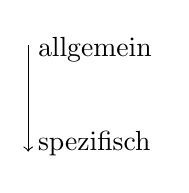
\begin{tikzpicture}
\node[right] at (0,0){spezifisch};
\node[right] at (0,1.2){allgemein};
\draw[<-] (0,-.1)--(0,1.25);
%\draw[<-] (0,.3)--(0,1);
\end{tikzpicture}

\end{minipage}

\begin{itemize}
	\item Notation verschiedener \textbf{Kontexte}:
	\begin{itemize}
		\item Silbengrenze: \$ oder: Silbenanfang: $_\sigma[$ und Silbenende: $]_\sigma$
		\item betonte Silbe: \textprimstress$\sigma$
		\item Koda: \underline{\quad}$_{\textsubscript{K}}$
		\item Morphemgrenze ($=$ Morphemanfang bzw.\ -ende): $+$
		\item Wortgrenze: \#
		\item \{ \dots\ ; \dots\ \} Liste von Kontexten, von denen nur einer gegeben sein muss
	\end{itemize}

\end{itemize}

\end{frame}


%%%%%%%%%%%%%%%%%%%%%%%%%%%%%%%%%
\subsection{Hausaufgabe}
%%%%%%%%%%%%%%%%%%%%%%%%%%%%%%%%%

\begin{frame}
\frametitle{Hausaufgabe}
\begin{itemize}
	\item[1.] Ordnen Sie die Artikulationsorte und -organe (Buchstaben) den entsprechenden Bezeichnungen (Klammern) zu.
	
\begin{minipage}{0.48\textwidth}
	\begin{figure}
		\centering
		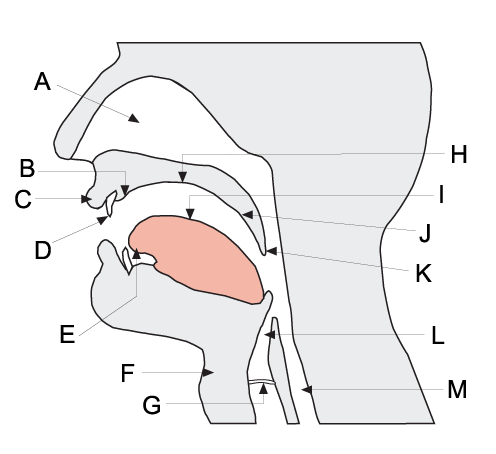
\includegraphics[scale=0.33]{material/04phonoatonomy}
	\end{figure}
\end{minipage}
\hfill
\begin{minipage}{0.4\textwidth}
	
		(~~) Stimmritze (glottal)\\
		(~~) Kehlkopf (laryngal)\\
		(~~) Zahndamm (alveolar)\\
		(~~) Nasenraum (nasal)\\
		(~~) harter Gaumen (palatal)\\
		(~~) Zähne (dental)\\
		(~~) weicher Gaumen (velar)\\
		(~~) Zungenrücken (dorsal)\\
		(~~) Halszäpfchen (uvular)\\
		(~~) Lippen (labial)\\
		(~~) Zungenspitze (apikal)
\end{minipage}

\end{itemize}
\end{frame}


%%%%%%%%%%%%%%%%%%%%%%%%%%%%%%%%
\begin{frame}{Hausaufgabe}
\begin{itemize}
	\item[2.] Welcher Laut passt jeweils nicht in die folgenden Reihen?\\
                  Begründen Sie Ihre Entscheidungen.
	
	\ea \label{ex:03aHA2}
		\ea \textipa{[b]}, \textipa{[z]}, \textipa{[a]}, \textipa{[g]}, \textipa{[v]}, \textipa{[p]}, \textipa{[u]}
		\ex \textipa{[t]}, \textipa{[s]}, \textipa{[n]}, \textipa{[\c{c}]}, \textipa{[l]}, \textipa{[d]}, \textipa{[r]}
		\ex \textipa{[f]}, \textipa{[s]}, \textipa{[x]}, \textipa{[h]}, \textipa{[r]}, \textipa{[z]}
		\ex \textipa{[N]}, \textipa{[m]}, \textipa{[k]}, \textipa{[g]}
		\ex \textipa{[m]}, \textipa{[b]}, \textipa{[N]}, \textipa{[p]}
		\z
	\z
	
	\item[3.] Geben Sie die \textbf{phonologische Repräsentation} der folgenden Wörter und \textbf{verschiedene phonetische Realisierungen} (\zB im Paradigma) an und \textbf{erläutern} Sie anschließend den \textbf{Unterschied} zwischen letzteren.
	
	\ea \label{ex:03aHA3}
		\ea Dieb
		\ex König
		\ex eng
		\z
	\z
	
\end{itemize}

\end{frame}


%%%%%%%%%%%%%%%%%%%%%%%%%%%%%%%%%
\begin{frame}{Hausaufgabe}

\begin{itemize}
	\item[4.] Bestimmen Sie, ob es sich bei den folgenden Lautkombinationen um Affrikaten handeln kann. Begründen Sie Ihre Entscheidungen.
	
	\ea \label{ex:03aHA4}
		\ea \textipa{[kl]}
		\ex \textipa{[pf]}
		\ex \textipa{[st]}
		\ex \textipa{[tr]}
		\ex \textipa{[ts]}
		\z
	\z
	
\end{itemize}

\end{frame}


%%%%%%%%%%%%%%%%%%%%%%%%%%%%%%%%%
\iftoggle{ha-loesung}{
	%%%%%%%%%%%%%%%%%%%%%%%%%%%%%%%%%%
%% HA 1 - 03a Phonologie
%%%%%%%%%%%%%%%%%%%%%%%%%%%%%%%%%%

\begin{frame}
\frametitle{Hausaufgabe -- Lösung}
\begin{itemize}
	\item[1.] Ordnen Sie die Artikulationsorte und -organe (Buchstaben) den entsprechenden Bezeichnungen (Klammern) zu.
	
	\begin{minipage}{0.48\textwidth}
		\begin{figure}
			\centering
			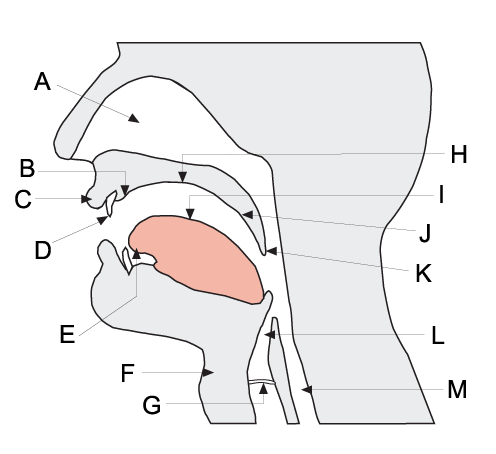
\includegraphics[scale=0.33]{material/04phonoatonomy}
		\end{figure}
	\end{minipage}
	\hfill
	\begin{minipage}{0.4\textwidth}
		
		(\visible<2->{\alertgreen{G}}) Stimmritze (glottal)\\
		(\visible<3->{\alertgreen{F}}) Kehlkopf (laryngal)\\
		(\visible<4->{\alertgreen{B}}) Zahndamm (alveolar)\\
		(\visible<5->{\alertgreen{A}}) Nasenraum (nasal)\\
		(\visible<6->{\alertgreen{H}}) harter Gaumen (palatal)\\
		(\visible<7->{\alertgreen{D}}) Zähne (dental)\\
		(\visible<8->{\alertgreen{J}}) weicher Gaumen (velar)\\
		(\visible<9->{\alertgreen{I}}) Zungenrücken (dorsal)\\
		(\visible<10->{\alertgreen{K}}) Halszäpfchen (uvular)\\
		(\visible<11->{\alertgreen{C}}) Lippen (labial)\\
		(\visible<12->{\alertgreen{E}}) Zungenspitze (apikal)
	\end{minipage}
	
\end{itemize}
\end{frame}


%%%%%%%%%%%%%%%%%%%%%%%%%%%%%%%%
\begin{frame}{Hausaufgabe -- Lösung}
\begin{itemize}
	\item[2.] Welcher Laut passt jeweils nicht in die folgenden Reihen?\\Begründen Sie Ihre Entscheidungen.
	
\begin{exe}
	\exr{ex:03aHA2}
\settowidth\jamwidth{XXXXXXXXXXXXXXXXXXXXXXXt}
	\begin{xlist}
		\ex \textipa{[b]}, \textipa{[z]}, \textipa{[a]}, \textipa{[g]}, \textipa{[v]}, \textipa{[p]}, \textipa{[u]} \loesung{2}{\textipa{[p]} (nicht sth., sondern stl.)}
		\ex \textipa{[t]}, \textipa{[s]}, \textipa{[n]}, \textipa{[\c{c}]}, \textipa{[l]}, \textipa{[d]}, \textipa{[r]} \loesung{3}{\textipa{[ç]} (nicht alveolar, sondern palatal)}
		\ex \textipa{[f]}, \textipa{[s]}, \textipa{[x]}, \textipa{[h]}, \textipa{[r]}, \textipa{[z]}
		\loesung{4}{\textipa{[r]} (kein Frikativ, sondern Vibrant)}
		\ex \textipa{[N]}, \textipa{[m]}, \textipa{[k]}, \textipa{[g]}
		\loesung{5}{\textipa{[k]} (nicht sth., sondern stl.)}\loesung{6}{oder: \textipa{[m]} (nicht velar, sondern labial)}
		\ex \textipa{[m]}, \textipa{[b]}, \textipa{[N]}, \textipa{[p]}
		\loesung{7}{\textipa{[N]} (nicht labial, sondern velar)} \loesung{8}{oder: \textipa{[p]} (nicht sth., sondern stl.)}
	\end{xlist}
\end{exe}
	
\end{itemize}
\end{frame}


%%%%%%%%%%%%%%%%%%%%%%%%%%%%%%%%
\begin{frame}{Hausaufgabe -- Lösung}
\begin{itemize}
	\item[3.] Geben Sie die \textbf{phonologische Repräsentation} der folgenden Wörter und \textbf{verschiedene phonetische Realisierungen} (\zB im Paradigma) an und \textbf{erläutern} Sie anschließend den \textbf{Unterschied} zwischen letzteren.
	
\begin{exe}
	\exr{ex:03aHA3}
	\settowidth\jamwidth{XXXXXXXXXXXXXXXXXXXXXXXXXXXXXXXXXXXXXXt}
	\begin{xlist}
		\ex Dieb
		\loesung{2}{\textipa{/di:b/}: \textipa{[di:p], [di:.bə]} -- Auslautverhärtung des \textipa{/b/} in der Koda}
		\ex König
		\loesung{3}{\textipa{/k\o :nıg/}: \textipa{[k\super h\o:.nıç], [k\super h\o:.nı.gə]} --} \loesung{3}{Spirantisierung des \textipa{/g/} in der Koda}
		\ex eng
		\loesung{4}{\textipa{/εng/}: \textipa{[PεN]}, \textipa{[PENk]} --}
		
		\loesung{4}{ g-Tilgung bzw. (dialektal) Auslautverhärtung}
	\end{xlist}
\end{exe}

\end{itemize}

\end{frame}


%%%%%%%%%%%%%%%%%%%%%%%%%%%%%%%%%
\begin{frame}{Hausaufgabe -- Lösung}

\begin{itemize}
	\item[4.] Bestimmen Sie, ob es sich bei den folgenden Lautkombinationen um Affrikaten handeln kann. Begründen Sie Ihre Entscheidungen.

\begin{exe}	
	\exr{ex:03aHA4}
\settowidth\jamwidth{XXXXXXXXXXXXXXXXXXXXXXXXXXXXXXXXXXXXXXX}
	\begin{xlist}
		\ex \textipa{[kl]} \loesung{2}{keine Affrikate (Zweitglied ist kein Frikativ)}
		\ex \textipa{[pf]} \loesung{3}{Affrikate (Verbindung aus Plosiv und homorganem Frikativ)}
		\ex \textipa{[st]} \loesung{4}{keine Affrikate (Plosiv ist Zweitglied)}
		\ex \textipa{[tr]} \loesung{5}{keine Affrikate (Zweitglied ist kein Frikativ)}
		\ex \textipa{[ts]} \loesung{6}{Affrikate (Verbindung aus Plosiv und homorganem Frikativ)}
	\end{xlist}
\end{exe}

\end{itemize}

\end{frame}



}
%%%%%%%%%%%%%%%%%%%%%%%%%%%%%%%%%



%% -*- coding:utf-8 -*-

%%%%%%%%%%%%%%%%%%%%%%%%%%%%%%%%%%%%%%%%%%%%%%%%%%%%%%%%%


\def\insertsectionhead{\refname}
\def\insertsubsectionhead{}

\huberlinjustbarfootline


\ifpdf
\else
\ifxetex
\else
\let\url=\burl
\fi
\fi
\begin{multicols}{2}
{\tiny
%\beamertemplatearticlebibitems

\bibliography{gkbib,bib-abbr,biblio}
\bibliographystyle{unified}
}
\end{multicols}





%% \section{Literatur}
%% \begin{frame}[allowframebreaks]
%% \frametitle{Literatur}
%% 	\footnotesize

%% \bibliographystyle{unified}

%% 	%German
%% %	\bibliographystyle{deChicagoMyP}

%% %	%English
%% %	\bibliographystyle{chicago} 

%% 	\bibliography{gkbib,bib-abbr,biblio}
	
%% \end{frame}


\end{document}

